\chapter{Rappresentazione delle molecole}

Fino ad ora abbiamo parlato del modo in cui gli atomi si legano per raggiungere uno stato più stabile, tuttavia ancora non abbiamo un modo per rappresentarne graficamente la struttura e la geometria. \\

Andiamo allora a introdurre le strutture di Lewis, per rappresentare lo scheletro della molecola, e la teoria VSEPR, per rappresentare la geometria. 

\section{Strutture di Lewis}

Una struttura di Lewis\mkeyword{struttura di Lewis} è una rappresentazione bidimensionale della molecola nella quale si indicano gli atomi, i legami che li uniscono e i doppietti elettronici non condivisi. Essa non fornisce alcuna informazione sulla geometria, ma ne costituisce il punto di partenza obbligato.

\subsection{Procedura di costruzione}

La costruzione si articola in quattro passi.

Si disegna anzitutto lo scheletro della molecola, stabilendo quali atomi siano legati fra loro. A tal fine sono utili tre criteri: un atomo presente in un solo esemplare occupa di norma la posizione centrale; l'atomo centrale è in genere il meno elettronegativo; le strutture risultanti sono spesso simmetriche.

Si calcola in secondo luogo il numero complessivo di elettroni di valenza, sommando i contributi di tutti gli atomi e tenendo conto dell'eventuale carica dello ione. Si sottraggono quindi due elettroni per ciascun legame semplice tracciato, e i rimanenti si distribuiscono come doppietti liberi sugli atomi periferici, a completare il loro ottetto.

Qualora al termine di tale distribuzione l'atomo centrale non raggiunga l'ottetto, si convertono doppietti liberi degli atomi periferici in legami multipli, oppure, per gli elementi a partire dal terzo periodo, si ricorre all'espansione dell'ottetto.\\

Nel pentacloruro di fosforo il fosforo espande l'ottetto.
Nel difluoruro di carbonile $COF_2$ il carbonio non può espandere l'ottetto e lo completa mediante un legame doppio con l'ossigeno. Nell'anidride carbonica il carbonio forma due legami doppi.


\begin{center}
\scalebox{0.8}{
\begin{tabular}{c@{\hspace{2.2em}}c@{\hspace{2.2em}}c}
 
% ================= PCl5 =================
\begin{tikzpicture}[baseline=(P.base)]
  \atomo{P}{0,0}{P}
  \atomo{Ca}{0,1.72}{Cl}   \atomo{Cb}{0,-1.72}{Cl}
  \atomo{Ce1}{-1.48,0}{Cl}
  \atomo{Ce2}{1.32,0.66}{Cl}  \atomo{Ce3}{1.32,-0.66}{Cl}
  \legame{P}{Ca}{1}{2pt}  \legame{P}{Cb}{1}{2pt}
  \legame{P}{Ce1}{1}{2pt} \legame{P}{Ce2}{1}{2pt} \legame{P}{Ce3}{1}{2pt}
  \doppietto{Ca}{0}\doppietto{Ca}{120}\doppietto{Ca}{180}
  \doppietto{Cb}{0}\doppietto{Cb}{180}\doppietto{Cb}{250}
  \doppietto{Ce1}{90}\doppietto{Ce1}{180}\doppietto{Ce1}{270}
  \doppietto{Ce2}{30}\doppietto{Ce2}{100}\doppietto{Ce2}{-60}
  \doppietto{Ce3}{-30}\doppietto{Ce3}{-100}\doppietto{Ce3}{60}
\end{tikzpicture}
&
% ================= COF2 =================
\begin{tikzpicture}[baseline=(C.base)]
  \atomo{C}{0,0}{C}
  \atomo{O}{0,1.30}{O}
  \atomo{F1}{-1.20,-0.72}{F}  \atomo{F2}{1.20,-0.72}{F}
  \legame{C}{O}{2}{3pt}
  \legame{C}{F1}{1}{2pt} \legame{C}{F2}{1}{2pt}
  \doppietto{O}{35}\doppietto{O}{145}
  \doppietto{F1}{90}\doppietto{F1}{180}\doppietto{F1}{265}
  \doppietto{F2}{90}\doppietto{F2}{0}\doppietto{F2}{275}
\end{tikzpicture}
&
% ================= CO2 =================
\begin{tikzpicture}[baseline=(C.base)]
  \atomo{C}{0,0}{C}
  \atomo{Oa}{-1.35,0}{O}  \atomo{Ob}{1.35,0}{O}
  \legame{C}{Oa}{2}{3pt} \legame{C}{Ob}{2}{3pt}
  \doppietto{Oa}{120}\doppietto{Oa}{240}
  \doppietto{Ob}{60}\doppietto{Ob}{-60}
\end{tikzpicture}
\\[1.4ex]
$\mathrm{PCl_5}$ & $\mathrm{COF_2}$ & $\mathrm{CO_2}$
\end{tabular}
}
\end{center}


\subsection{Carica formale}

La procedura descritta può condurre a più strutture formalmente ammissibili. Per stabilire quale sia preferibile si ricorre a un criterio contabile.

Si definisce carica formale\mkeyword{carica formale} di un atomo in una molecola la differenza fra il numero di elettroni di valenza dell'atomo isolato e il numero di elettroni ad esso assegnati nella struttura, computando per intero i doppietti liberi e per metà gli elettroni di ciascun legame.

\begin{equation}
    q_f = n_{\text{valenza}} - n_{\text{liberi}} - \frac{1}{2}\,n_{\text{legame}}
    \label{eq:carica_formale}
\end{equation}

La \eqref{eq:carica_formale} presuppone dunque una ripartizione perfettamente paritaria degli elettroni di legame, il che equivale a trascurare le differenze di elettronegatività: la carica formale non è pertanto una carica reale, bensì uno strumento di confronto fra strutture. La somma delle cariche formali di tutti gli atomi è nulla per una molecola neutra e pari alla carica complessiva per uno ione.

Le strutture si ordinano per plausibilità secondo i criteri seguenti, elencati in ordine di importanza decrescente: sono preferibili le strutture in cui tutte le cariche formali siano nulle, e in mancanza di queste quelle che presentano il maggior numero di atomi a carica formale nulla; le cariche formali negative devono collocarsi sugli atomi più elettronegativi e quelle positive sui meno elettronegativi; le cariche devono essere quanto più possibile piccole in valore assoluto, ed eventuali cariche su atomi adiacenti devono avere segno opposto.

\subsection{Risonanza}

Per talune molecole il criterio della carica formale non è sufficiente, poiché la struttura che esso individua risulta in contrasto con l'esperienza.

L'ozono ne è l'esempio più semplice: entrambe le strutture di Lewis che si possono scrivere prevedono un legame semplice e uno doppio, e quindi due legami di lunghezza diversa, mentre sperimentalmente essi risultano identici. Analogamente il protossido di azoto ammette due strutture, delle quali quella preferibile secondo le cariche formali non corrisponde a ciò che si osserva.

La difficoltà non risiede nella scelta fra le strutture, bensì nel formalismo stesso: la molecola reale non corrisponde ad alcuna di esse.\\

Si dice ibrido di risonanza\mkeyword{ibrido di risonanza} la struttura reale di una molecola per la quale è possibile scrivere più strutture di Lewis differenti soltanto per la disposizione dei doppietti elettronici, essendo identica quella dei nuclei. Le singole strutture si dicono forme limite e si collegano con una doppia freccia.\\

\begin{center}
\begin{tikzpicture}[scale=1.3]

% --- Struttura 1 ---
\atomo{OL1}{-1.0,0}{O}
\atomo{OC1}{0,0.5}{O}
\atomo{OR1}{1.0,0}{O}

\legame{OL1}{OC1}{2}{6pt}
\legame{OC1}{OR1}{1}{6pt}

\doppietto{OL1}{180}
\doppietto{OL1}{135}
\doppietto{OL1}{225}
\node at ($(OC1)+(0,0.32)$) {$+$};
\doppietto{OR1}{0}
\doppietto{OR1}{45}
\doppietto{OR1}{90}
\doppietto{OR1}{135}
\node[right] at ($(OR1)+(0.32,0)$) {$-$};

% --- Freccia di risonanza ---
\draw[<->, line width=0.6pt] (1.7,0.25) -- (2.5,0.25);

% --- Struttura 2 ---
\atomo{OL2}{3.2,0}{O}
\atomo{OC2}{4.2,0.5}{O}
\atomo{OR2}{5.2,0}{O}

\legame{OL2}{OC2}{1}{6pt}
\legame{OC2}{OR2}{2}{6pt}

\doppietto{OR2}{0}
\doppietto{OR2}{-45}
\doppietto{OR2}{45}
\node at ($(OC2)+(0,0.32)$) {$+$};
\doppietto{OL2}{180}
\doppietto{OL2}{135}
\doppietto{OL2}{90}
\doppietto{OL2}{225}
\node[left] at ($(OL2)+(-0.32,0)$) {$-$};

\end{tikzpicture}
\end{center}

\newpage

L'ibrido di risonanza non è una miscela di molecole diverse, né una molecola che oscilli nel tempo fra le forme limite: queste ultime non hanno esistenza fisica, e la molecola reale è un'unica entità intermedia. La denominazione, di origine storica, è sotto questo aspetto infelice. Nel linguaggio degli orbitali molecolari il fenomeno si descrive dicendo che gli elettroni $\pi$ occupano un orbitale delocalizzato esteso su più atomi: la risonanza è il modo in cui la teoria di Lewis, che sa rappresentare soltanto legami localizzati, tenta di rendere conto della delocalizzazione.\\

La condizione perché due strutture siano forme limite è che la disposizione dei nuclei sia la medesima e che varino soltanto le posizioni dei doppietti. Le strutture $H - N = C = O$ e $N \equiv C - O - H$ non sono pertanto forme di risonanza, bensì isomeri distinti, poiché nel passare dall'una all'altra un atomo di idrogeno cambia posizione.\\

L'ibrido di risonanza possiede infine energia inferiore a quella di ciascuna delle forme limite, per la ragione generale che la delocalizzazione, offrendo agli elettroni una regione più estesa, ne abbassa l'energia. Tale differenza prende il nome di energia di risonanza\mkeyword{energia di risonanza} ed è la causa della particolare stabilità dei sistemi coniugati.

\subsection{Limiti della rappresentazione}

Le strutture di Lewis costituiscono uno strumento contabile di grande efficacia, ma non una descrizione fisica del legame. Oltre alle eccezioni alla regola dell'ottetto già discusse, se ne segnalano due limiti ulteriori.

Il primo riguarda i radicali: nel monossido di azoto, con undici elettroni di valenza, l'ottetto non è raggiungibile e resta un elettrone spaiato, il che ne fa una specie assai reattiva.

Il secondo, più profondo, riguarda l'ossigeno molecolare, per il quale nessuna struttura di Lewis è in grado di rendere conto simultaneamente dell'ordine di legame e del paramagnetismo osservati. Ciò indica che la rappresentazione mediante coppie localizzate, per quanto utile, non esaurisce la descrizione del legame chimico.

\newpage

\section{Teoria VSEPR}

Le strutture di Lewis indicano quali atomi siano legati fra loro, ma nulla dicono sulla disposizione nello spazio: essendo rappresentazioni piane, esse non costituiscono un modello geometrico. La teoria VSEPR, dall'inglese \emph{valence shell electron pair repulsion}, colma tale lacuna a partire da un unico principio.\\

I doppietti elettronici del guscio di valenza dell'atomo centrale, essendo dotati di carica dello stesso segno, si respingono mutuamente e si dispongono nello spazio alla massima distanza angolare possibile\mkeyword{teoria VSEPR}.\\

Si tratta di un criterio puramente elettrostatico e geometrico, che non richiede alcuna informazione sulla natura degli orbitali coinvolti. La sua semplicità non ne compromette l'efficacia: le geometrie previste risultano in ottimo accordo con quelle misurate per la gran parte dei composti degli elementi dei blocchi $s$ e $p$.

\subsection{Numero sterico}

Si definisce numero sterico\mkeyword{numero sterico} dell'atomo centrale la somma del numero di atomi ad esso legati e del numero di doppietti liberi che esso possiede.

\begin{equation}
    SN = n_{\text{atomi legati}} + n_{\text{doppietti liberi}}
    \label{eq:numero_sterico}
\end{equation}

Nella \eqref{eq:numero_sterico} un legame multiplo si conta come un solo elemento, poiché i doppietti che lo costituiscono occupano la medesima regione dello spazio e si comportano, ai fini della repulsione, come un'unica entità. L'anidride carbonica, pur presentando due legami doppi, ha pertanto numero sterico pari a due.

Il numero sterico determina univocamente la disposizione dei doppietti attorno all'atomo centrale, ossia la geometria elettronica\mkeyword{geometria elettronica}:

\begin{center}
    \begin{tabular}{ccc}
        \toprule
        $SN$ & Geometria elettronica & Angolo \\
        \midrule
        2 & lineare                  & $180^\circ$ \\
        3 & trigonale planare        & $120^\circ$ \\
        4 & tetraedrica              & $109{,}5^\circ$ \\
        5 & bipiramidale trigonale   & $120^\circ$ e $90^\circ$ \\
        6 & ottaedrica               & $90^\circ$ \\
        \bottomrule
    \end{tabular}
\end{center}

\subsection{Geometria molecolare}

Occorre a questo punto una distinzione essenziale. I doppietti liberi occupano una posizione e ne determinano la disposizione complessiva, ma non sono osservabili sperimentalmente: la forma di una molecola è definita unicamente dalle posizioni dei nuclei.\\

Si dice geometria molecolare\mkeyword{geometria molecolare} la disposizione spaziale dei soli atomi, ottenuta dalla geometria elettronica ignorando i doppietti liberi.\\

Si adotta comunemente la notazione $AX_nE_m$, nella quale $A$ indica l'atomo centrale, $X$ gli atomi legati in numero $n$ ed $E$ i doppietti liberi in numero $m$, sicché $SN = n+m$.

\begin{center}
    \begin{tabular}{clllc}
        \toprule
        $SN$ & Notazione & Geometria molecolare & Esempio & Angolo \\
        \midrule
        2 & $AX_2$    & lineare                & $CO_2$    & $180^\circ$ \\
        \midrule
        3 & $AX_3$    & trigonale planare      & $BF_3$    & $120^\circ$ \\
          & $AX_2E$   & angolare               & $SO_2$    & $<120^\circ$ \\
        \midrule
        4 & $AX_4$    & tetraedrica            & $CH_4$    & $109{,}5^\circ$ \\
          & $AX_3E$   & piramidale trigonale   & $NH_3$    & $107^\circ$ \\
          & $AX_2E_2$ & angolare               & $H_2O$    & $104{,}5^\circ$ \\
        \midrule
        5 & $AX_5$    & bipiramidale trigonale & $PCl_5$   & \\
          & $AX_4E$   & ad altalena            & $SF_4$    & \\
          & $AX_3E_2$ & a T                    & $ClF_3$   & \\
          & $AX_2E_3$ & lineare                & $XeF_2$   & $180^\circ$ \\
        \midrule
        6 & $AX_6$    & ottaedrica             & $SF_6$    & $90^\circ$ \\
          & $AX_5E$   & piramidale quadrata    & $BrF_5$   & \\
          & $AX_4E_2$ & quadrata planare       & $XeF_4$   & $90^\circ$ \\
        \bottomrule
    \end{tabular}
\end{center}

Si osservi che molecole con il medesimo numero sterico possono avere forme del tutto diverse: metano, ammoniaca e acqua hanno tutte $SN = 4$ e geometria elettronica tetraedrica, ma risultano rispettivamente tetraedrica, piramidale e angolare a seconda di quanti vertici del tetraedro siano occupati da doppietti liberi anziché da atomi.

\begin{figure}[h]
  \centering
  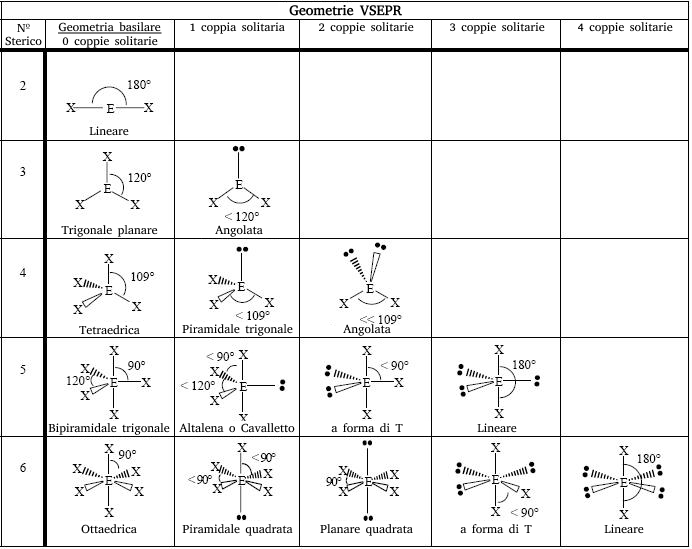
\includegraphics[width=1.0\linewidth]{foto/VSEPR.png}
  \label{fig:etichetta}
\end{figure}

\subsection{Deviazioni dagli angoli ideali}

Gli angoli riportati si osservano esattamente soltanto quando tutte le posizioni sono equivalenti. Le deviazioni si spiegano osservando che un doppietto libero è trattenuto da un solo nucleo e risulta pertanto più diffuso angolarmente, mentre un doppietto di legame è compresso lungo l'asse internucleare dall'attrazione di due nuclei. Ne segue la gerarchia delle repulsioni

\begin{equation}
    \text{lp--lp} \; > \; \text{lp--bp} \; > \; \text{bp--bp}
    \label{eq:gerarchia_vsepr}
\end{equation}

nella quale si sono indicati con lp i doppietti liberi e con bp quelli di legame. Ciascun doppietto libero comprime dunque gli angoli fra i legami, e l'effetto è cumulativo: nella serie $CH_4$, $NH_3$, $H_2O$ l'angolo passa da $109{,}5^\circ$ a $107^\circ$ e infine a $104{,}5^\circ$.

Un effetto analogo, seppure meno marcato, è prodotto dai legami multipli, che essendo più ricchi di densità elettronica esercitano una repulsione maggiore di quella dei legami semplici.\\

La bipiramide trigonale è l'unica fra le geometrie considerate in cui le posizioni non sono equivalenti. Le posizioni assiali possiedono tre vicini a $90^\circ$, quelle equatoriali soltanto due, e risentono pertanto di una repulsione maggiore: ne segue che i legami assiali sono più lunghi e più deboli, e soprattutto che i doppietti liberi occupano sempre per primi le posizioni equatoriali. È questa regola a generare la sequenza di forme ad altalena, a T e lineare al crescere del numero di doppietti.

\subsection{Limiti della teoria}

La teoria VSEPR fornisce previsioni corrette per la quasi totalità dei composti degli elementi dei blocchi $s$ e $p$, ma presenta alcune limitazioni.

Essa non è applicabile ai metalli di transizione, nei quali la geometria è determinata dagli effetti del campo dei leganti sugli orbitali $d$ piuttosto che dalla semplice repulsione fra doppietti, né alle molecole prive di un atomo centrale identificabile. Si riscontrano inoltre eccezioni sistematiche negli alogenuri degli elementi pesanti del gruppo $2A$, quali $CaF_2$ e $BaF_2$, i quali risultano angolari in fase gassosa anziché lineari come previsto.

Va infine ricordato che la VSEPR predice la geometria ma non ne fornisce una giustificazione in termini di struttura elettronica: essa non sostituisce la trattazione mediante orbitali, bensì ne costituisce una scorciatoia predittiva di notevole comodità.
